% Copyright (c) 2018 Robert Carnell

\documentclass[11pt,letter]{book}

\usepackage[T1]{fontenc}

% Fonts added for the book
\usepackage[bitstream-charter]{mathdesign} % use the bitstream-charter True Type font

% ---- Gramps Packages ----
%\usepackage[latin1]{inputenc}%
\usepackage[latin1,utf8]{inputenc}%
\usepackage{graphicx}% Extended graphics support
\usepackage{longtable}% For multi-page tables
\usepackage{calc}% For some calculations
\usepackage{ifthen}% For table width calculations
\usepackage{ragged2e}% For left aligning with hyphenation
\usepackage{wrapfig}% wrap pictures in text

% Packages added for the book
\usepackage[all]{genealogytree} % genealogy-tree package for trees
\usepackage{draftwatermark} % create draft watermark
% watermark modifications
\SetWatermarkText{DRAFT}
\SetWatermarkScale{1}
\SetWatermarkColor[rgb]{0.9,0.9,0.9}

% --------- Gramps Section ----------

% Depending on your LaTeX installation, the margins may be too
% narrow.  This can be corrected by uncommenting the following
% two lines and adjusting the width appropriately. The example
% removes 0.5in from each margin. (Adds 1 inch to the text)
%\addtolength{\oddsidemargin}{-0.5in}%
%\addtolength{\textwidth}{1.0in}%

% Vertical spacing between paragraphs:
% take one of three possibilities or modify to your taste:
\setlength{\parskip}{1.0ex plus0.2ex minus0.2ex}%
%\setlength{\parskip}{1.5ex plus0.3ex minus0.3ex}%
%\setlength{\parskip}{2.0ex plus0.4ex minus0.4ex}%

% Vertical spacing between lines:
% take one of three possibilities or modify to your taste:
\renewcommand{\baselinestretch}{1.0}%
%\renewcommand{\baselinestretch}{1.1}%
%\renewcommand{\baselinestretch}{1.2}%

% Indentation; substitute for '1cm' of gramps, 2.5em is right for 12pt
% take one of three possibilities or modify to your taste:
\newlength{\grbaseindent}%
%\setlength{\grbaseindent}{3.0em}%
\setlength{\grbaseindent}{2.5em}%
%\setlength{\grbaseindent}{2.0em}%


% -------------------------------------------------------------
% New lengths, counters and commands for calculations in tables
% -------------------------------------------------------------

\newlength{\grtabwidth}%
\newlength{\grtabprepos}%
\newlength{\grreqwidth}%
\newlength{\grtempwd}%
\newlength{\grmaxwidth}%
\newlength{\grprorated}%
\newlength{\grxwd}%
\newlength{\grwidthused}%
\newlength{\grreduce}%
\newlength{\grcurcolend}%
\newlength{\grspanwidth}%
\newlength{\grleadlabelwidth}%
\newlength{\grminpgindent}%
\newlength{\grlistbacksp}%
\newlength{\grpictsize}%
\newlength{\grmaxpictsize}%
\newlength{\grtextsize}%
\newlength{\grmaxtextsize}%
\newcounter{grtofixcnt}%
\newcounter{grxwdcolcnt}%
%
%
\newcommand{\grinitlength}[2]{%
  \ifthenelse{\isundefined{#1}}%
    {\newlength{#1}}{}%
  \setlength{#1}{#2}%
}%
%
\newcommand{\grinittab}[2]{%    #1: tabwidth, #2 = 1.0/anz-cols
  \setlength{\grtabwidth}{#1}%
  \setlength{\grprorated}{#2\grtabwidth}%
  \setlength{\grwidthused}{0em}%
  \setlength{\grreqwidth}{0em}%
  \setlength{\grmaxwidth }{0em}%
  \setlength{\grxwd}{0em}%
  \setlength{\grtempwd}{0em}%
  \setlength{\grpictsize}{0em}%
  \setlength{\grmaxpictsize}{0em}%
  \setlength{\grtextsize}{0em}%
  \setlength{\grmaxtextsize}{0em}%
  \setlength{\grcurcolend}{0em}%
  \setcounter{grxwdcolcnt}{0}%
  \setcounter{grtofixcnt}{0}%  number of wide cols%
  \grinitlength{\grcolbega}{0em}% beg of first col
}%
%
\newcommand{\grmaxvaltofirst}[2]{%
  \ifthenelse{\lengthtest{#1 < #2}}%
    {\setlength{#1}{#2}}{}%
}%
%
\newcommand{\grsetreqfull}{%
  \grmaxvaltofirst{\grmaxpictsize}{\grpictsize}%
  \grmaxvaltofirst{\grmaxtextsize}{\grtextsize}%
}%
%
\newcommand{\grsetreqpart}[1]{%
  \addtolength{\grtextsize}{#1 - \grcurcolend}%
  \addtolength{\grpictsize}{#1 - \grcurcolend}%
  \grsetreqfull%
}%
%
\newcommand{\grdividelength}{%
 \setlength{\grtempwd}{\grtabwidth - \grwidthused}%
%    rough division of lengths:
%    if 0 < #1 <= 10: \grxwd = ~\grtempwd / grtofixcnt
%    otherwise: \grxwd =  \grprorated
 \ifthenelse{\value{grtofixcnt} > 0}%
  {\ifthenelse{\value{grtofixcnt}=1}%
                    {\setlength{\grxwd}{\grtempwd}}{%
    \ifthenelse{\value{grtofixcnt}=2}
                    {\setlength{\grxwd}{0.5\grtempwd}}{%
     \ifthenelse{\value{grtofixcnt}=3}
                    {\setlength{\grxwd}{0.333\grtempwd}}{%
      \ifthenelse{\value{grtofixcnt}=4}
                    {\setlength{\grxwd}{0.25\grtempwd}}{%
       \ifthenelse{\value{grtofixcnt}=5}
                    {\setlength{\grxwd}{0.2\grtempwd}}{%
        \ifthenelse{\value{grtofixcnt}=6}
                    {\setlength{\grxwd}{0.166\grtempwd}}{%
         \ifthenelse{\value{grtofixcnt}=7}
                    {\setlength{\grxwd}{0.143\grtempwd}}{%
          \ifthenelse{\value{grtofixcnt}=8}
                    {\setlength{\grxwd}{0.125\grtempwd}}{%
           \ifthenelse{\value{grtofixcnt}=9}
                    {\setlength{\grxwd}{0.111\grtempwd}}{%
            \ifthenelse{\value{grtofixcnt}=10}
                    {\setlength{\grxwd}{0.1\grtempwd}}{%
             \setlength{\grxwd}{\grprorated}% give up, take \grprorated%
    }}}}}}}}}}%
  \setlength{\grreduce}{0em}%
  }{\setlength{\grxwd}{0em}}%
}%
%
\newcommand{\grtextneedwidth}[1]{%
  \settowidth{\grtempwd}{#1}%
  \grmaxvaltofirst{\grtextsize}{\grtempwd}%
}%
%
\newcommand{\grcolsfirstfix}[5]{%
  \grinitlength{#1}{\grcurcolend}%
  \grinitlength{#3}{0em}%
  \grinitlength{#4}{\grmaxpictsize}%
  \grinitlength{#5}{\grmaxtextsize}%
  \grinitlength{#2}{#5}%
  \grmaxvaltofirst{#2}{#4}%
  \addtolength{#2}{2\tabcolsep}%
  \grmaxvaltofirst{\grmaxwidth}{#2}%
  \ifthenelse{\lengthtest{#2 < #4} \or \lengthtest{#2 < \grprorated}}%
    { \setlength{#3}{#2}%
      \addtolength{\grwidthused}{#2} }%
    { \stepcounter{grtofixcnt} }%
  \addtolength{\grcurcolend}{#2}%
}%
%
\newcommand{\grcolssecondfix}[4]{%
  \ifthenelse{\lengthtest{\grcurcolend < \grtabwidth}}%
    { \setlength{#3}{#2} }%
    { \addtolength{#1}{-\grreduce}%
      \ifthenelse{\lengthtest{#2 = \grmaxwidth}}%
        { \stepcounter{grxwdcolcnt}}%
        { \ifthenelse{\lengthtest{#3 = 0em} \and %
                       \lengthtest{#4 > 0em}}%
            { \setlength{\grtempwd}{#4}%
              \grmaxvaltofirst{\grtempwd}{\grxwd}%
              \addtolength{\grreduce}{#2 - \grtempwd}%
              \setlength{#2}{\grtempwd}%
              \addtolength{\grwidthused}{#2}%
              \addtocounter{grtofixcnt}{-1}%
              \setlength{#3}{#2}%
            }{}%
        }%
    }%
}%
%
\newcommand{\grcolsthirdfix}[3]{%
  \ifthenelse{\lengthtest{\grcurcolend < \grtabwidth}}%
    {}{ \addtolength{#1}{-\grreduce}%
        \ifthenelse{\lengthtest{#3 = 0em} \and %
                     \lengthtest{#2 < \grmaxwidth}}%
          { \ifthenelse{\lengthtest{#2 < 0.5\grmaxwidth}}%
              { \setlength{\grtempwd}{0.5\grxwd}%
                \grmaxvaltofirst{\grtempwd}{0.7\grprorated}}%
              { \setlength{\grtempwd}{\grxwd}}%
            \addtolength{\grreduce}{#2 - \grtempwd}%
            \setlength{#2}{\grtempwd}%
            \addtolength{\grwidthused}{#2}%
            \addtocounter{grtofixcnt}{-1}%
            \setlength{#3}{#2}%
          }{}%
      }%
}%
%
\newcommand{\grcolsfourthfix}[3]{%
  \ifthenelse{\lengthtest{\grcurcolend < \grtabwidth}}%
    {}{ \addtolength{#1}{-\grreduce}%
        \ifthenelse{\lengthtest{#3 = 0em}}%
          { \addtolength{\grreduce}{#2 - \grxwd}%
            \setlength{#2}{\grxwd}%
            \setlength{#3}{#2}%
          }{}%
      }%
}%
%
\newcommand{\grgetspanwidth}[4]{%
  \grinitlength{#1}{#3 - #2 + #4}%
}%
%
\newcommand{\tabheadstrutceil}{%
  \rule[0.0ex]{0.00em}{3.5ex}}%
\newcommand{\tabheadstrutfloor}{%
  \rule[-2.0ex]{0.00em}{2.5ex}}%
\newcommand{\tabrowstrutceil}{%
  \rule[0.0ex]{0.00em}{2.9ex}}%
\newcommand{\tabrowstrutfloor}{%
  \rule[-0.1ex]{0.00em}{2.0ex}}%
%
\newcommand{\grempty}[1]{}%
%
\newcommand{\graddvdots}[1]{%
  \hspace*{\fill}\hspace*{\fill}\raisebox{#1}{\vdots}%
}%
%
\newcommand{\grtabpgbreak}[4]{%
  #1 { \parbox[t]{ #2 - 2\tabcolsep}{\tabheadstrutceil\hspace*{\fill}%
  \raisebox{#4}{\vdots} #3{#4} \hspace*{\fill}\tabheadstrutfloor}}%
}%
%
\newcommand{\grcolpart}[3]{%
  #1 { \parbox[t]{ #2 - 2\tabcolsep}%
  {\tabrowstrutceil #3~\\[-1.6ex]\tabrowstrutfloor}}%
}%
%
\newcommand{\grminpghead}[2]{%
  \setlength{\grminpgindent}{#1\grbaseindent-\grlistbacksp}%
  \hspace*{\grminpgindent}%
  \ifthenelse{\not \lengthtest{#2em > 0em}}%
    {\begin{minipage}[t]{\textwidth -\grminpgindent}}%
    {\begin{minipage}[t]{\textwidth -\grminpgindent%
        -#2\grbaseindent -4\tabcolsep}}%
}%
%
\newcommand{\grminpgtail}{%
  \end{minipage}\parindent0em%
}%
%
\newcommand{\grlisthead}[1]{%
  \begin{list}{#1}%
    { \setlength{\labelsep}{0.5em}%
      \setlength{\labelwidth}{\grleadlabelwidth}%
      \setlength{\leftmargin}{\grlistbacksp}%
    }\item%
}%
%
\newcommand{\grlisttail}{%
  \end{list}%
}%
%
\newcommand{\grprepleader}[1]{%
  \settowidth{\grtempwd}{#1}%
  \ifthenelse{\lengthtest{\grtempwd > \grleadlabelwidth}}%
    { \setlength{\grleadlabelwidth}{\grtempwd}}{}%
  \setlength{\grlistbacksp}{\grleadlabelwidth + 1.0em}%
}%
%
\newcommand{\grprepnoleader}{%
  \setlength{\grleadlabelwidth}{0em}%
  \setlength{\grlistbacksp}{0em}%
}%
%
\newcommand{\grmkpicture}[4]{%
    \begin{wrapfigure}{r}{#2\grbaseindent}%
      \vspace{-6ex}%
      \begin{center}%
      \includegraphics[%
        width= #2\grbaseindent,%
        height= #3\grbaseindent,%
          keepaspectratio]%
        {#1}\\%
      {\RaggedRight\footnotesize#4}%
      \end{center}%
    \end{wrapfigure}%
    \settowidth{\grtempwd}{\footnotesize#4}%
    \setlength{\grxwd}{#2\grbaseindent}%
    \ifthenelse{\lengthtest{\grtempwd < 0.7\grxwd}}%
                    {\setlength{\grxwd}{1ex}}{%
      \ifthenelse{\lengthtest{\grtempwd < 1.2\grxwd}}%
                    {\setlength{\grxwd}{2ex}}{%
        \ifthenelse{\lengthtest{\grtempwd < 1.8\grxwd}}%
                    {\setlength{\grxwd}{6ex}}{%
          \ifthenelse{\lengthtest{\grtempwd < 2.0\grxwd}}%
                    {\setlength{\grxwd}{10ex}}{%
                     \setlength{\grxwd}{12ex}}%
                    }}}%
  \setlength{\grtempwd}{#3\grbaseindent + \grxwd}%
  \rule[-\grtempwd]{0pt}{\grtempwd}%
  \setlength{\grtabprepos}{-\grtempwd}%
}%

% -------------------- End Gramps Section ----------------------

\title{\bf Carnell-Rettgers Family Genealogy \\
       \large Volume VI - Descendants of Connell-Langston and Smith-Josey}
\author{Robert Carnell}
\date{\today}

\begin{document}
\frontmatter
\maketitle
\clearpage

\begingroup
\parindent 0pt
\parskip
\baselineskip
Copyright \textcopyright{} 2018 Robert Carnell

All rights reserved.  This book or any portion thereof may not be reproduced or used in any manner whatsoever with the express written permission of the author except for the use or brief quotations in a book review or genealogical research.
\endgroup
\clearpage

\tableofcontents
\mainmatter

\chapter{Introduction}

The first generation of descendants of the Connell-Langston and Smith-Josey families were part of the Greatest Generation.  They were born during the Great Depression (29 Oct 1929 - abt 1938) and many fought in or were greatly affected by World War II (1 Sep 1939 in Europe, 7 Dec 1941 in the U.S. to 14 Aug 1945 V-J Day).  These dramatic events shaped their outlook and instilled qualities in them that were essential to their success and the success of future generations.

\begin{itemize}
\item The Greatest Generation 1901-1924
\item Silent 1925-1945
\item Baby Boomers 1946-1964
\item Generation X 1965-1980
\end{itemize}

\chapter{Descendants of William Connell and Nellie Langston}

\section{Tree}

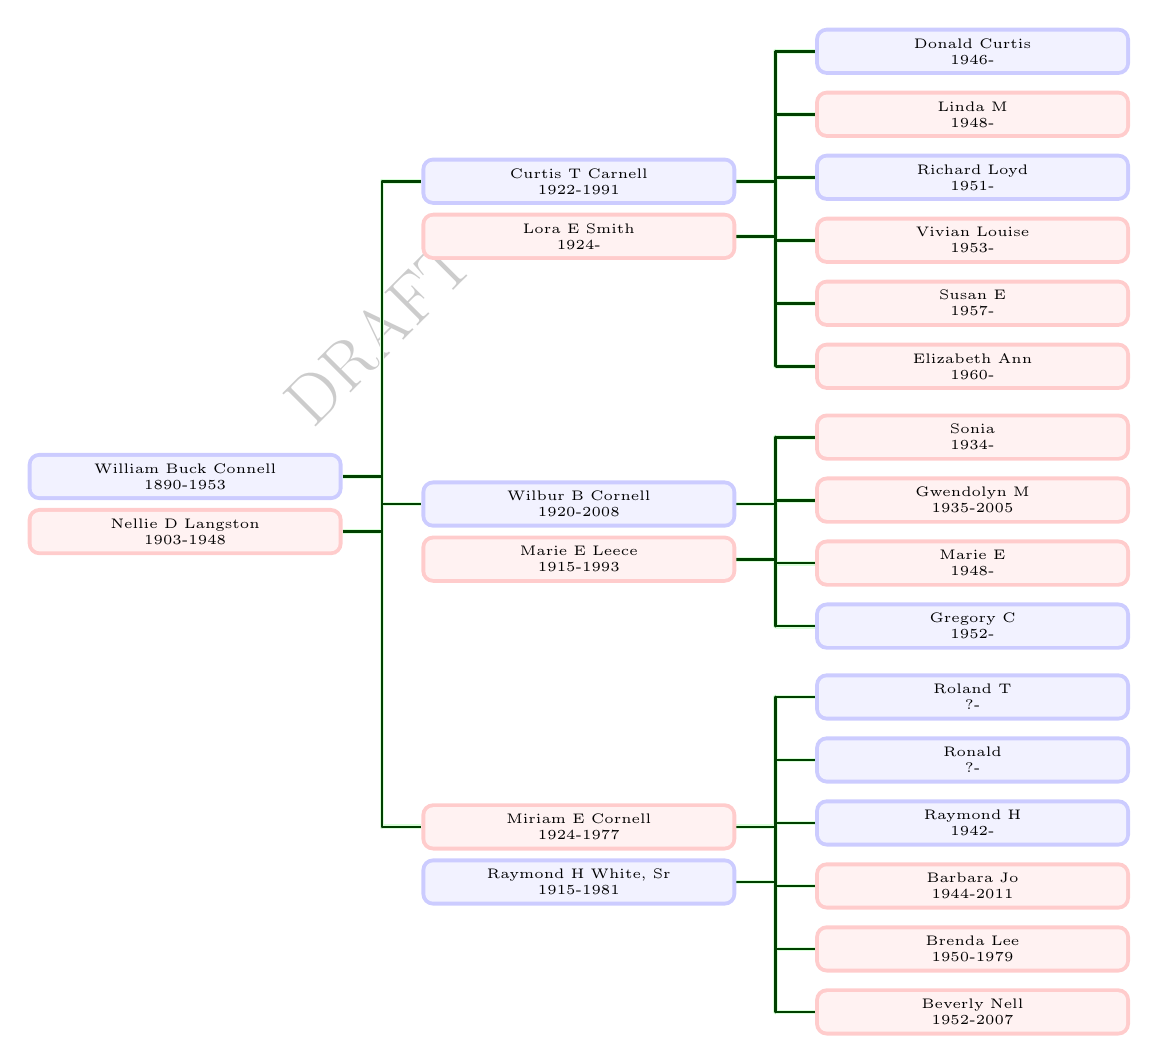
\begin{tikzpicture}
	\genealogytree[
		template=signpost,
		timeflow=right,
		node size=0.6cm, 
		level size=4.0cm,
		tcbset={male/.style={colframe=blue!20, colback=blue!5},
			female/.style={colframe=red!20, colback=red!5}},
		box={fit basedim=8pt, boxsep=1pt, no shadow}
	]{
		child{
			p[male]{William Buck Connell\\1890-1953}
			g[female]{Nellie D Langston\\1903-1948}
			child{
				g[male]{Curtis T Carnell\\1922-1991}
				p[female]{Lora E Smith\\1924-}
				c[male]{Donald Curtis\\1946-}
				c[female]{Linda M\\1948-}
				c[male]{Richard Loyd\\1951-}
				c[female]{Vivian Louise\\1953-}
				c[female]{Susan E\\1957-}
				c[female]{Elizabeth Ann\\1960-}
			}
			child{
				g[male]{Wilbur B Cornell\\1920-2008}
				p[female]{Marie E Leece\\1915-1993}
				c[female]{Sonia\\1934-}
				c[female]{Gwendolyn M\\1935-2005}
				c[female]{Marie E\\1948-}
				c[male]{Gregory C\\1952-}
			}
			child{
				g[female]{Miriam E Cornell\\1924-1977}
				p[male]{Raymond H White, Sr\\1915-1981}
				c[male]{Roland T\\?-}
				c[male]{Ronald\\?-}
				c[male]{Raymond H\\1942-}
				c[female]{Barbara Jo\\1944-2011}
				c[female]{Brenda Lee\\1950-1979}
				c[female]{Beverly Nell\\1952-2007}
			}
		}
	}
\end{tikzpicture}

\section{Genealogy}

\input{../tex_output/det_descendant_report_Connell_mod.tex}

\chapter{Descendants of K Smith and J Josey}

\section{Tree}

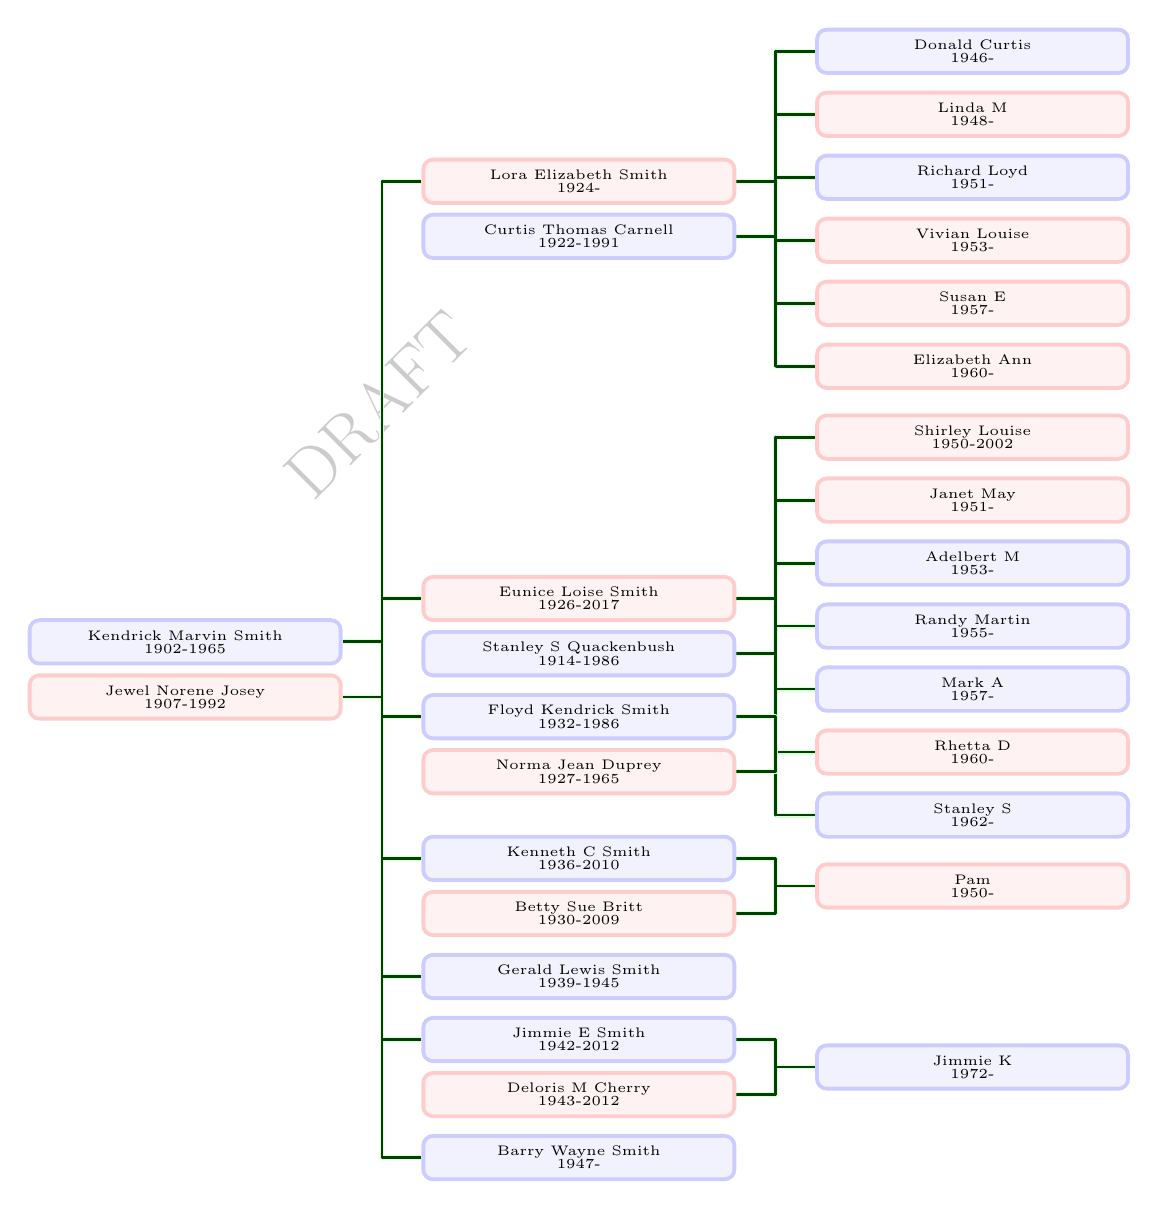
\begin{tikzpicture}
	\genealogytree[
		template=signpost,
		timeflow=right, 
		node size=0.6cm, 
		level size=4.0cm,
		tcbset={male/.style={colframe=blue!20, colback=blue!5},
			female/.style={colframe=red!20, colback=red!5}},
		box={fit basedim=8pt, boxsep=2pt, no shadow}
	]{
		child{
			g[male]{Kendrick Marvin Smith\\1902-1965}
			p[female]{Jewel Norene Josey\\1907-1992}
			child{
				g[female]{Lora Elizabeth Smith\\1924-}
				p[male]{Curtis Thomas Carnell\\1922-1991}
				c[male]{Donald Curtis\\1946-}
				c[female]{Linda M\\1948-}
				c[male]{Richard Loyd\\1951-}
				c[female]{Vivian Louise\\1953-}
				c[female]{Susan E\\1957-}
				c[female]{Elizabeth Ann\\1960-}
			}
			child{				
				g[female]{Eunice Loise Smith\\1926-2017}
				p[male]{Stanley S Quackenbush\\1914-1986}
				c[female]{Shirley Louise\\1950-2002}
				c[female]{Janet May\\1951-}
				c[male]{Adelbert M\\1953-}
				c[male]{Randy Martin\\1955-}
				c[male]{Mark A\\1957-}
				c[female]{Rhetta D\\1960-}
				c[male]{Stanley S\\1962-}
			}
			child{
				g[male]{Floyd Kendrick Smith\\1932-1986}
				p[female]{Norma Jean Duprey\\1927-1965}
			}
			child{
				g[male]{Kenneth C Smith\\1936-2010}
				p[female]{Betty Sue Britt\\1930-2009}
				c[female]{Pam\\1950-}
			}
			c[male]{Gerald Lewis Smith\\1939-1945}
			child{
				g[male]{Jimmie E Smith\\1942-2012}
				p[female]{Deloris M Cherry\\1943-2012}
				c[male]{Jimmie K\\1972-}
			}
			c[male]{Barry Wayne Smith\\1947-}
		}
	}
\end{tikzpicture}

\section{Genealogy}

\input{../tex_output/det_descendant_report_Smith_mod.tex}

\chapter{Endnotes}

\section{Connell-Langston Endnotes}

\footnotesize

\input{../tex_output/det_descendant_report_Connell_mod_notes.tex}

\normalsize

\section{Smith-Josey Endnotes}

\footnotesize

\input{../tex_output/det_descendant_report_Smith_mod_notes.tex}

\normalsize

\end{document}

